\documentclass[10pt,twocolumn]{article}

\usepackage{times}
\usepackage{fullpage}
\usepackage{color}
\usepackage{natbib}
\usepackage{graphicx}

\newcommand{\todo}[1]{\noindent{\textcolor{red}{\{{\bf TODO:}  #1\}}}}

\begin{document}

\title{\bf RABIT: A Robust AllReduce and Broadcast Interface}
\author{Tianqi Chen\hspace{0.5in}Ignacio Cano\hspace{0.5in}Tianyi Zhou \\\\
Department of Computer Science \& Engineering \\
University of Washington\\
}
\date{}
\maketitle
\thispagestyle{empty}

\begin{abstract}

AllReduce is an abstraction commonly used for solving machine learning problems. It is an operation where every node starts with a local value and ends up with an aggregate global result.
MPI package provides an AllReduce implementation. Though it has been widely adopted, it is somewhat limited; it lacks fault tolerance and cannot run easily on existent systems, such as Spark, Hadoop, etc.

In this work, we propose RABIT, an AllReduce library suitable for distributed machine learning algorithms that overcomes the aforementioned drawbacks; it is fault-tolerant and can easily run on top of existent systems.

\end{abstract}

\section{Introduction}
Distributed machine learning is an active research area that has seen an incredible grow in recent years. Several approaches have been proposed, e.g. parameter server abstraction, graph approaches, among others \cite{paramServer,DuchiAW12,Zinkevich,Dekel,Low}. The closest example to our work is proposed by Agarwal et al. \cite{Agarwal}, in which they have a tree-shape communication infrastructure that efficiently accumulates and broadcasts values to every node involved in a computation.



\section{AllReduce}

In AllReduce settings, nodes are organized in a tree structure. Each node holds a portion of the data and computes some values on it. Those values are passed up the tree and aggregated, until a global aggregate value is calculated in the root node (reduce). The global value is then passed down to all other nodes (broadcast). 

Figure \ref{allreduce} shows an example of an AllReduce sum operation. The leaf nodes passed data to their parents (interior nodes). Such interior nodes compute an intermediate aggregate and pass the value to the root, which in turn computes the final aggregate and then passes back the result to every node in the cluster.

\begin{figure}[tb]
\centering
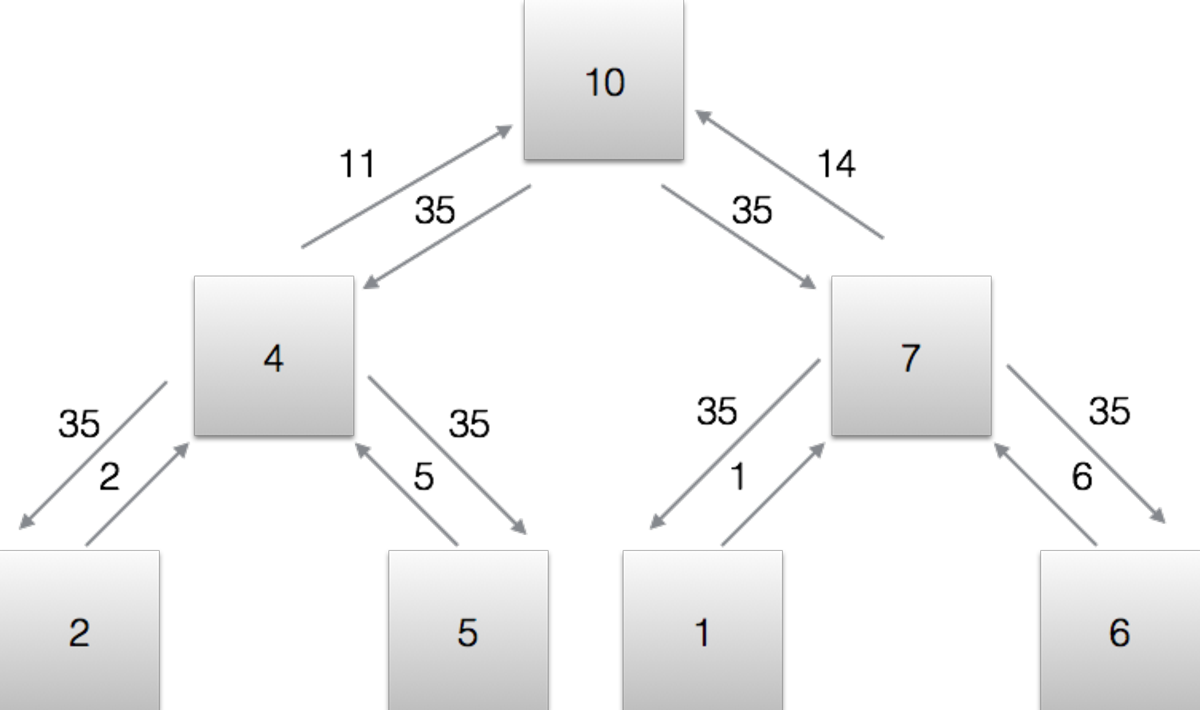
\includegraphics[width=0.7\columnwidth]{fig/allreduce.pdf}
\caption{AllReduce example}
\label{allreduce}
\end{figure}


\section{RABIT}


\subsection{Design Goals}

The design of RABIT was motivated by the following needs:

\begin{enumerate}
  \item \emph{Distributed}: machine learning algorithms are inherently iterative and computation intensive. Given the vast amount of data they can work on, it may be intractable to perform all the processing on a single machine. Instead, we want to divide the computation into different nodes, each one would be in charge of computing statistics on some portion of the data, and then a combination step would take place, where all those independent local solutions will be aggregated into a single result.
  \item \emph{Scalability}: we want our solution to handle a growing amount of work in a capable manner, i.e. we should be able to accommodate to data and computation growth by adding more nodes.
  \item \emph{Fault Tolerance}: we assume an environment where failures happen, either machines can go down or communication failures occur. Given the computation intensive nature of machine learning problems, we want to be able to continue operating properly in the event of a failure, instead of starting the process all over again.
  \item \emph{Programmability}: we want to provide a clean interface that can be easily used by programmers. With few lines of code, they should be able to have a fault-tolerant AllReduce implementation.
  \item \emph{Re-usability}: we want to build a library based on a few low-level primitives, e.g. AllReduce and Broadcast operations. Higher level abstractions, e.g. Recover operation, should reuse those basic building blocks.
  \item \emph{Communication Efficiency}: closely related to the \emph{Scalability} goal. We want to send as few control messages as possible. We also want to reuse existent connections in order to avoid starting overheads.
  \item \emph{Footprint}: we want to have a low memory footprint while running as well as provide a lightweight footprint library.
\end{enumerate}

\subsection{Interface}

\todo{add sync module interface, example of how to use the library}

\section{Evaluation}

\todo{add benchmarks and our results}


\section{Conclusion \& Future Work}

With the exponential increase of data on the web, it becomes critical to build systems that can process information efficiently in order to extract value out of it. Several abstractions have been proposed to address those requirements. In this project, we focus on the AllReduce abstraction. We propose an efficient and fault tolerant version that can be used together with existent big data analytics systems, such as Spark, Hadoop, etc.
We compare our solution to MPI's AllReduce implementation, and show that the performance difference between the two is negligible considering our version is fault tolerant.
\todo{improve this}

\subsection*{Acknowledgments}
Thanks to Arvind Krishnamurthy and the CSE550 teaching staff for their guidance and support during the quarter.

\bibliography{rabit}
\bibliographystyle{abbrv} 

\end{document}

